% \documentclass[preprint]{kcc}
\documentclass{kcc}


%%%%%%%%%%%%%%%%%%%%%%%%%%%%%%%%%%%%%%%%%%%%%%%
% include additional packages you need to use
%%%%%%%%%%%%%%%%%%%%%%%%%%%%%%%%%%%%%%%%%%%%%%%
% graphic, float package
\usepackage{graphicx}		% for setting images
\usepackage{float}			% for float objects
\usepackage{subfloat}		
\usepackage{subfigure}		% for adding several figures in a figure environment
\usepackage{lscape}			% for landscape type images or tables


\usepackage{enumitem}

% for compact section title spacing
% \usepackage[compact]{titlesec}


% mathmetical presentation
\usepackage{gensymb}
\usepackage{amsmath}
\usepackage{amssymb}
\usepackage{amsthm}
\usepackage{exscale}
\usepackage{textcomp}		% extra symbols


% for circled number
\newcommand{\cl}[1]{\textcircled{\scriptsize #1}}


% package for using algorithmic presentation
\usepackage{algorithmic}
\usepackage{algorithm}
% customize algorithmic environment
\renewcommand{\algorithmicrequire}{\makebox[40px]{\hfill\textbf{Input :}}}
\renewcommand{\algorithmicensure}{\makebox[40px]{\hfill\textbf{Output :}}}

% array and table presentation
\usepackage{array}
\usepackage{tabulary}
\usepackage{multirow}
\usepackage[table]{xcolor}
\usepackage{ctable}
\usepackage{booktabs}		% for typesetting tables at the level of publication		
							% do not use vertical rule
							
							\usepackage{times}
\usepackage{CJKutf8}
\usepackage{mathrsfs}
\usepackage{verbatim}
\usepackage{amsfonts}
\usepackage{xspace}
\usepackage{xcolor}
\usepackage{url}
\usepackage{balance}
\usepackage{booktabs}
\usepackage{multirow}
\usepackage{rotating}
\usepackage{fancyvrb}
\usepackage{lastpage}
\usepackage{alltt}
\usepackage{etoolbox}
\usepackage{cleveref} % After hyperref, listings
\usepackage{fancyhdr}
\usepackage{listings}

\usepackage{caption}


% set title, author, abstract
\title{Fine dust prediction using Convloutional Long Short-Term\\ Memory Model and geological matrix}
\author{
}
\engtitle{} \engauthor{
}
\abstract{
This paper proposes a new prediction method for the increasing amount of ultrafine dust in Korea.
Unlike predictions using existing simple statistics, we use matrix that take into account the geological location of China and Korea. In addition, LSTM(Long Short-Term Memory) was adopted to use existing time series fine dust data. The results of this method are compared with the existing data, and the problems to be solved in the future are suggested.
}

\begin{document}

\maketitle

\section{Introduction}

The fine dust in Korea is increasing rapidly as the year goes by.
Furthermore, as more and more small fine dust (PM 2.5) increases, it is hard to see with the naked eye.In this situation, prediction of fine dust is becoming very important.However, current methods of prediction are less accurate.
There have been many studies to solve this problem.

Previous researches have mainly focused on one area, and some of them are based on the assumption of the reason for the high concentration of fine dust, and the reason for this is the relationship between the fine dust and the reason.
However, as in many weather forecasts, there are many anomalies that can not be explained by reason alone.

So, we have predicted by building up a geological matrix consisting of fine dust except for the data and other additional factors for the last three years, deviating from predicting using decades old data which were mainly used.



\section{Background and related work}

\textbf{\textit{Convolution}} In mathematics (and, in particular, functional analysis) convolution is a mathematical operation on two functions (f and g); it produces a third function, that is typically viewed as a modified version of one of the original functions, giving the integral of the pointwise multiplication of the two functions as a function of the amount that one of the original functions is translated. Convolution is similar to cross-correlation. It has applications that include probability, statistics, computer vision, natural language processing, image and signal processing, engineering, and differential equations.

\textbf{\textit{RNN(Recurrent Neural Network)}} A recurrent neural network (RNN) is a class of artificial neural network where connections between units form a directed cycle. This creates an internal state of the network which allows it to exhibit dynamic temporal behavior. Unlike feedforward neural networks, RNNs can use their internal memory to process arbitrary sequences of inputs. This makes them applicable to tasks such as unsegmented connected handwriting recognition or speech recognition.

\textbf{\textit{LSTM}}
Long short-term memory (LSTM) is a recurrent neural network (RNN) architecture (an artificial neural network) proposed in 1997 by Sepp Hochreiter and Jürgen Schmidhuber and further improved in 2000 by Felix Gers et al. Like most RNNs, a LSTM network is universal in the sense that given enough network units it can compute anything a conventional computer can compute, provided it has the proper weight matrix, which may be viewed as its program. Unlike traditional RNNs, an LSTM network is well-suited to learn from experience to classify, process and predict time series when there are time lags of unknown size and bound between important events. Relative insensitivity to gap length gives an advantage to LSTM over alternative RNNs and hidden Markov models and other sequence learning methods in numerous applications. Among other successes, LSTM achieved the best known results in natural language text compression, unsegmented connected handwriting recognition, and in 2009 won the ICDAR handwriting competition. LSTM networks have also been used for automatic speech recognition, and were a major component of a network that in 2013 achieved a record 17.7\% phoneme error rate on the classic TIMIT natural speech dataset. As of 2016, major technology companies including Google, Apple, Microsoft, and Baidu are using LSTM networks as fundamental components in new products. For example, Google uses LSTM for speech recognition on the smartphone, for the smart assistant Allo, and for Google Translate. Apple uses LSTM for the "Quicktype" function on the iPhone and for Siri. Amazon uses LSTM for Amazon Alexa.

\textbf{\textit{Process Data}}
We were able to get a lot of fine dust information from Korea, but China was a closed country, so only five large cities were available. We decided to write data from three of the five cities, Shenyang, Shanghai and Beijing, which are closest to Korea. The PM2.5 (fine dust less than 2.5?m in diameter) data by city in Korea was quite empty. That part has been replaced by data from the nearest area.

\textbf{\textit{Related Studies}}
Originally, We tried to use a convolutional neural network, but I decided that a convolutional recurrent neural network would be more appropriate. So, We studied about hyper parameter tuning. Most machine learning algorithms have many settings that need to be specified by researchers or technicians. These tuning options are called hyper parameters and are used to adjust the algorithm when optimizing performance or balancing bias bias and variance variance. For example, How to set padding in Convolutional neural network. And Fine dust data are shown every hour so How to cut off time and whether to put the average value into the part or the broken part is to put the maximum value or the minimum value. All of this is an important part of improving accuracy. 

\section{Experiment enviroment}

The experimental environment is shown in Figure ~\ref{fig:xeon} and is an Intel i7-based 8-core machine. I used the GTX1080 as the GPU.
\begin{figure}[h]
  \begin{center}
     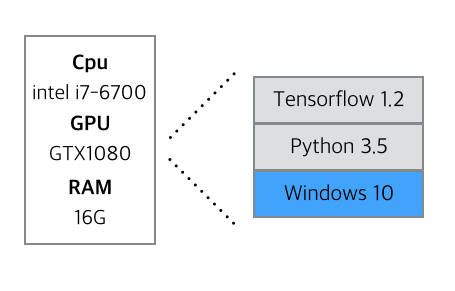
\includegraphics[width=0.3\textwidth]{fig/env.png}
  \end{center}
  \caption{Environment}
  \label{fig:xeon}
\end{figure}

For the measurement environment, software of the same version as Table ~\ref{tab:config} was used.
And the input data is collected by using the data that is open to the Internet.

\begin{table}[h!]
  \caption{Software version and input data}
  \centering
  \small
  \begin{tabular}{l l l l l} \toprule
    OS & Tool & Python & Tensorflow & input data\\
    \midrule
    Windows 10 & Tensorflow & 3.5.2 & 1.2.0 & fine dust data \\
    \bottomrule
  \end{tabular}
  \label{tab:config}
\end{table}

\section{Fine dust prediction}
This section explains how this differs from the existing rule-based approach and details its model. We modeled the existing methods and theories appropriately.
The table~\ref{tab:Company} shows the name of the popular forecasting model, whether it is public or not, and information about the model name.

\begin{table}[h!]
  \caption{Existing model}
  \centering
  \scriptsize 
  \begin{tabular}{l l l l l} \toprule 
    Name & Public & Model name \\
    \midrule
    Cams & No & Copernicus Atrmosphere Monitoring model \\
    \midrule
    SILAM & Yes & System for Integrated model\\
    \midrule
    SPRINTARS & Yes & Spectral Radiation-Transport model\\
    \midrule
    PANDA & No & -\\
    \bottomrule
  \end{tabular}
  \label{tab:Company}
\end{table}

\subsection{Approach}

Most of the publicly available models address the causal relationship of how the actual fine dust is generated. But we decided to pay more attention to the results more simply. A two-dimensional matrix was generated based on the actual PM2.5 data. In this process, we tried to solve the relation between Chinese fine dust and Korean fine dust by borrowing not only Korean data but also Chinese data. We create a data matrix based on the day and plot it as follows Figure~\ref{fig:data}. Convolution is applied by applying a 3x3 kernel based on this 90x90 matrix. We try to predict by applying such inputs to the LSTM model.
Our hidden layer size was 10, and the total number of steps was 760 days. Stride did not skip data at 1, and the optimizer used adamoptimizer to learn to minimize loss.
\begin{figure}[h]
  \begin{center}
     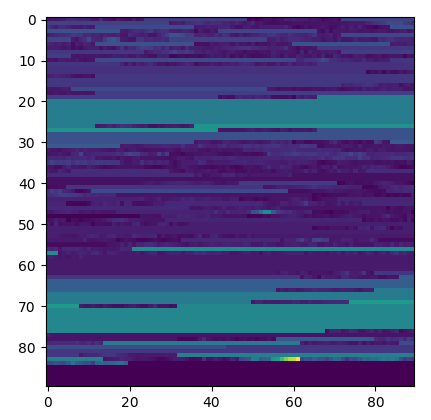
\includegraphics[width=0.3\textwidth]{fig/data.png}
  \end{center}
  \caption{Data matrix image}
  \label{fig:data}
\end{figure}

To illustrate the model, we can briefly explain this Figure~\ref{fig:model} . Convolve the basic data in the upper left corner to create new data. It then learns through the recurrent network and creates new predictions with the learned weights. 

\begin{figure}[h]
  \begin{center}
     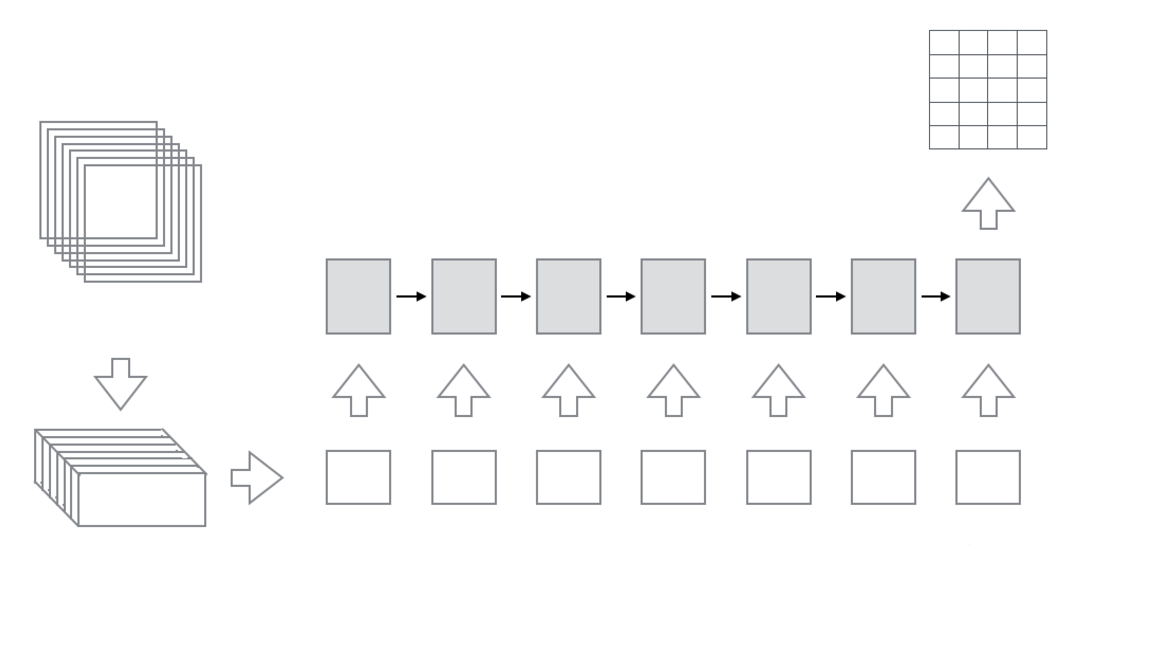
\includegraphics[width=0.3\textwidth]{fig/model.png}
  \end{center}
  \caption{Model summary}
  \label{fig:model}
\end{figure}

\section{Conclusion and Future Work}
We predicted a total of 7 matrix based on the model we trained and compared with the rest of the commonly used methods against existing measured data.
You can see from the Table ~\ref{tab:result}. Amazingly disappointing results came out. The predictability of all existing models is over 80\%, while the model we trained has not even exceeded 65\%.
So I thought about what was lacking and there were various problems.

\begin{table}[h!]
  \caption{Result}
  \centering
  \scriptsize 
  \begin{tabular}{l l l l l} \toprule 
    Name & 1day & 3day & 7day \\
    \midrule
    Cams & 89\% &  90\% & 90\%\\
    \midrule
    SILAM & 91\% & 88\% & 85\%\\
    \midrule
    SPRINTARS & 85\% & 87\% & 91\%\\
    \midrule
    PANDA & 88\% & 85\% & 83\%\\
    \midrule
    Out Method & 62\% & 52\% & 43\% \\
    \bottomrule
  \end{tabular}
  \label{tab:result}
\end{table}

First, the data was too small. Our original plan was to split the 24 hour day into hours and model it. However, there was some damage to the acquired data, and there was also a problem with the coverage of the data, so We arbitrarily subdivided the sections to create the input data every day. As a result, the total data did not exceed 1000, and based on the year, the data was based on a little more than two years of data.

Second, We thought of too few factors when constructing the model. We thought that China was the biggest problem, and we thought about this model with the assumption that all the results would be right if we had an association with China. However, as a result, we noticed that there are many other factors as well as China, so we need to model it.




\bibliographystyle{ieeetr}
\begin{thebibliography}{7}
\bibitem{n1}
\newblock F. Bastien, P. Lamblin, R. Pascanu, J. Bergstra, I. Goodfellow, A. Bergeron, N. Bouchard, D. WardeFarley,
and Y. Bengio. Theano: New features and speed improvements. Deep Learning and Unsupervised
Feature Learning NIPS 2012 Workshop, 2012.
\bibitem{n2}
\newblock Y. Bengio, I. Goodfellow, and A. Courville. Deep Learning. Book in preparation for MIT Press, 2015.
\bibitem{n3}
\newblock J. Bergstra, O. Breuleux, F. Bastien, P. Lamblin, R. Pascanu, G. Desjardins, J. Turian, D. Warde-Farley,
and Y. Bengio. Theano: a CPU and GPU math expression compiler. In Scipy, volume 4, page 3. Austin,
TX, 2010.
\bibitem{n4}
\newblock R. Bridson. Fluid Simulation for Computer Graphics. Ak Peters Series. Taylor \& Francis, 2008.

\end{thebibliography}

%\bibliographystyle{ieeetr}
%\bibliography{ref}

\end{document}
